\documentclass{article}
\usepackage[utf8]{inputenc}
\usepackage{amssymb}
\usepackage{amsmath}
\usepackage{enumitem}
\usepackage{tabto}
\usepackage[]{algorithm2e}
\usepackage{textcomp}
\usepackage{siunitx}
\usepackage{graphicx}
\usepackage{wrapfig}
\usepackage{siunitx}
\usepackage{subcaption}
\graphicspath{{images/}}

\title{Master Project}
\author{Rufat Eyvazli }
\date{June 2020}

\begin{document}

\begin{title} \\
    \begin{center} 
         \textbf{PaNaRuf}\\~\\
 		 Stitching Multiple Radial-Symmetric Fisheye Images for Obtaining \ang{360}x\ang{180} Panoramic Image\\~\\
        
    Rufat Eyvazli\\
    stu213430@mail.uni-kiel.de\\
    MSc Computer Science\\
    CAU Kiel \\~\\
    10 June, 2020
    \end{center}
\end{title}
\section*{Abstract} This report mainly describes the workflow and challanges of PaNaRuf; a software that achieves \ang{360} x \ang{180} spherical/equirectangular panoramic image by stitching multiple overlapping (e.g., 50\%) radial-symmetric fisheye images each with field of view $\geq \ang{180}$. The sections in the workflow basically cover important mathematics behind, the necessary algorithms used, evaluations/experiments observed and the detailed discussions about sucesses and failures of the software. 

\section*{Introduction}
Today, spherical panoramic projection is the most accurate panoramic projection method that is able to cover \ang{360} horizontal angle and \ang{180} vertical angle from the reference point of the projection. One can approach the same accuracy with cylindrical panoramic projection as well, but some data, especially in top and bottom, will be lost. On the other hand, the spherical panorama achieves 2:1-ratio image covering 360 x 180 degrees. The only problem with this projection is some distortions in top and bottom of the view. This is acceptable because it is theoretically impossible to project all points in sphere to a plane without distortions [1].

PaNaRuf creates spherical panoramic image with ratio \ang{360} x \ang{180} by stittching multiple neighbouring fisheye images with good overlap (e.g, 50\%). Firstly, the software derives multiple rectilinear images (along with the corresponding camera parameters) from each of the fisheye images. Then, it finds best relations among the set of rectilinear images. Accordingly, it updates the necessary rotation matrices. Finally, spherical panoramic projection is applied to each rectilinear image and the warped images are stitched using blending. The detailed workflow achieving these, is well described in the next sections. \\~\\

\section*{Motivation}
Nowadays, such a software gains importance in many fields, especially when large field coverage is needed. For instance, when an astronaut needs all information of 360 degree around in the space, he/she can take multiple well-overlapping fisheye images, and can easily create spherical panoramic image using such a software. In addition to astronomy, there are many other fields where such program can be very useful: 3D computer graphics, advertisements, robotics, panoramic photography etc. This software can be considered as an alternative tool to omni-directional cameras specialized for 360 panorama images. It is as good as such cameras but the only expected errors can be observed in stittching due to estimations.

\section*{Workflow}
The whole pipeline that have been followed in the implementation of the program to achieve spherical panoramic image are listed below in sequential order:
\begin{itemize}
    \item Fisheye to rectilinear images
    \begin{itemize}
		\item A. Set corresponding camera parameters
    		\item B. Map points between pinhole and physical fisheye image
    \end{itemize} 
    \item Find relations among image sets
    \begin{itemize}
    		\item A. Extract features
    		\item B. Direct Linear Transform
    		\item C. RANSAC-based homography estimation
    		\item D. Update appropriate rotation matrices
    \end{itemize}
    \item Equirectangular/Spherical warping
    \begin{itemize}
		\item A. Forward mapping
		\item B. Backward mapping
    \end{itemize}  
    \item Stittching
    \item Evaluation
\end{itemize}
\ \\~\\

\section*{Fisheye to Rectilinear Images.}
Before passing to the technical explanations, we give the main idea of this section below:

All points in the fisheye image are un-projected to a unit-sphere. It is assumed that there is a virtual pinhole camera model at (0,0,0) and it looks  towards (0,0,1) on a unit sphere. Then rotating this camera, multiple rectilinear images are taken to cover all fields of sphere where the fisheye image points have been un-projected to. \\~\\
\textbf{A. Set corresponding camera parameters:}
\ \\
For an image taken in 3D, the corresponding 3 x 3 camera calibration/intrinsic matrix K,  3 x 3 camera rotation/extrinsic matrix R and 1 x 3 camera translation vector $t$ are set to create 3 x 4 camera matrix P where [2]:
\begin{center}
				$P = K[R | t]$
\end{center}
However, in this case, the camera is not translated but only rotated. Therefore, the translation vector t is neglected. So, for each taken rectilinear image, the corresponding camera calibration matrix K and camera rotation matrix R are created.\\~\\
\textit{Camera intrinsic parameter}:	
Camera calibration matrix K has 5 instrinsic parameters as indicated in the matrix below [2]: 
\begin{equation*}
    K = \begin{bmatrix}
			f_{x} & s & c_{x}\\
			0 & f_{y} & c_{y}\\
            0 & 0 & 1
			\end{bmatrix}
\end{equation*} 				
In general, $s$ represents skew coefficient between the sensor axis. However, in practice, it is usually neglected (set to 0). $c_{x}$ and $c_{y}$ represents the principal point which are set to half of width and half of height of the taken rectilinear image respectivelly. $f_{x}$ and $f_{y}$, on the other hand, stand for focal length in pixels and is computed as below:
\begin{center}
	$f = \cfrac{W}{2} \cdot (\ \tan \cfrac{\theta}{2} \ )^{-1}$
\end{center}
where $W$ represents sensor width and $\theta$ (in radian) represents field of view [2].

In the software, \ang{90} (converted to radian) has been chosen as both horizontal and vertical field of view and the resolution of each rectilinear image has been chosen as 300 x 300 by default.\\~\\
\textit{Camera extrinsic parameter}:
A rotation matrix R is usually decomposed into 3 different rotation matrices as 
$R =  R_{x} R_{y} R_{z}$ where $R_{x}$, $R_{y}$ and $R_{z}$ represent rotations around x,y and z axis respectively by $\alpha$ degree as defined below [3]:
\begin{equation*}
   \scriptstyle  R_{x}(\alpha) = \begin{bmatrix}
			1 & 0 & 0\\
			0 & \cos{\alpha} & -\sin{\alpha}\\
            0 & \sin{\alpha} & \cos{\alpha}
			\end{bmatrix}, \        
	R_{y}(\alpha) =  \begin{bmatrix}
			\cos{\alpha} & 0 & \sin{\alpha}\\
			0 & 1 & 0\\
            -\sin{\alpha} & 0 & \cos{\alpha}
			\end{bmatrix}, \ 
	R_{z}(\alpha) = \begin{bmatrix}
			\cos{\alpha} & -\sin{\alpha} & 0\\
			\sin{\alpha} & \cos{\alpha} & 0\\
            0 & 0 & 1
			\end{bmatrix}    
\end{equation*}
In PaNaRuf, no matter around which axis the camera is rotated, the corresponding angle is chosen as $\pm\ang{45}$ (converted to radian)\\~\\
Pinhole camera parameters are defined as described above but this is not enough. Additionally, the focal length $F$ of fisheye lens should be defined to un-project 2D fisheye image point to 3D points on unit-sphere and vice versa. $F$ can be determined using any of the projection model listed below[4]: 
\begin{center}
Equidistant: $r_{d} = F \theta$\\
\ \ \ \ \ \ \ Stereographic: $r_{d} = 2F \tan(\frac{\theta}{2})$\\
\ \ \ \ \ \ \ \ \ \ \ \ Equisolid: $r_{d} = 2F \sin(\frac{\theta}{2})$\\
\ \ \ \ \ Orthographic: $r_{d} = F \sin(\theta)$\\
\end{center}
where, $r_d$ is the radial distance from the principal point and $\theta$ is inclination angle (in radian) which measures the angular difference between the ray of light and the optical axis [4].

According to Xiaolong Li in [5], \textit{Equidistant} is the most widely used projection model. Therefore, in the software, this projection model is used to find the focal length $F$ as below: 
\begin{center}
    $F = \cfrac{0.5 \cdot N}{0.5 \cdot FOV} = \cfrac{N}{FOV} $ 
\end{center}
where N represents minimum dimension between width and height of fisheye image and FOV denotes field of view in radian. \\~\\
After describing all of the necessary definitions, several rectilinear images are obtained from a fisheye image by applying the following mapping procedure to each pixel of a rectilinear image.\\~\\
\textbf{B. Map points between pinhole and physical fisheye image :}
\ \\

\begin{wrapfigure}{r}{0.25\textwidth}
    \centering
    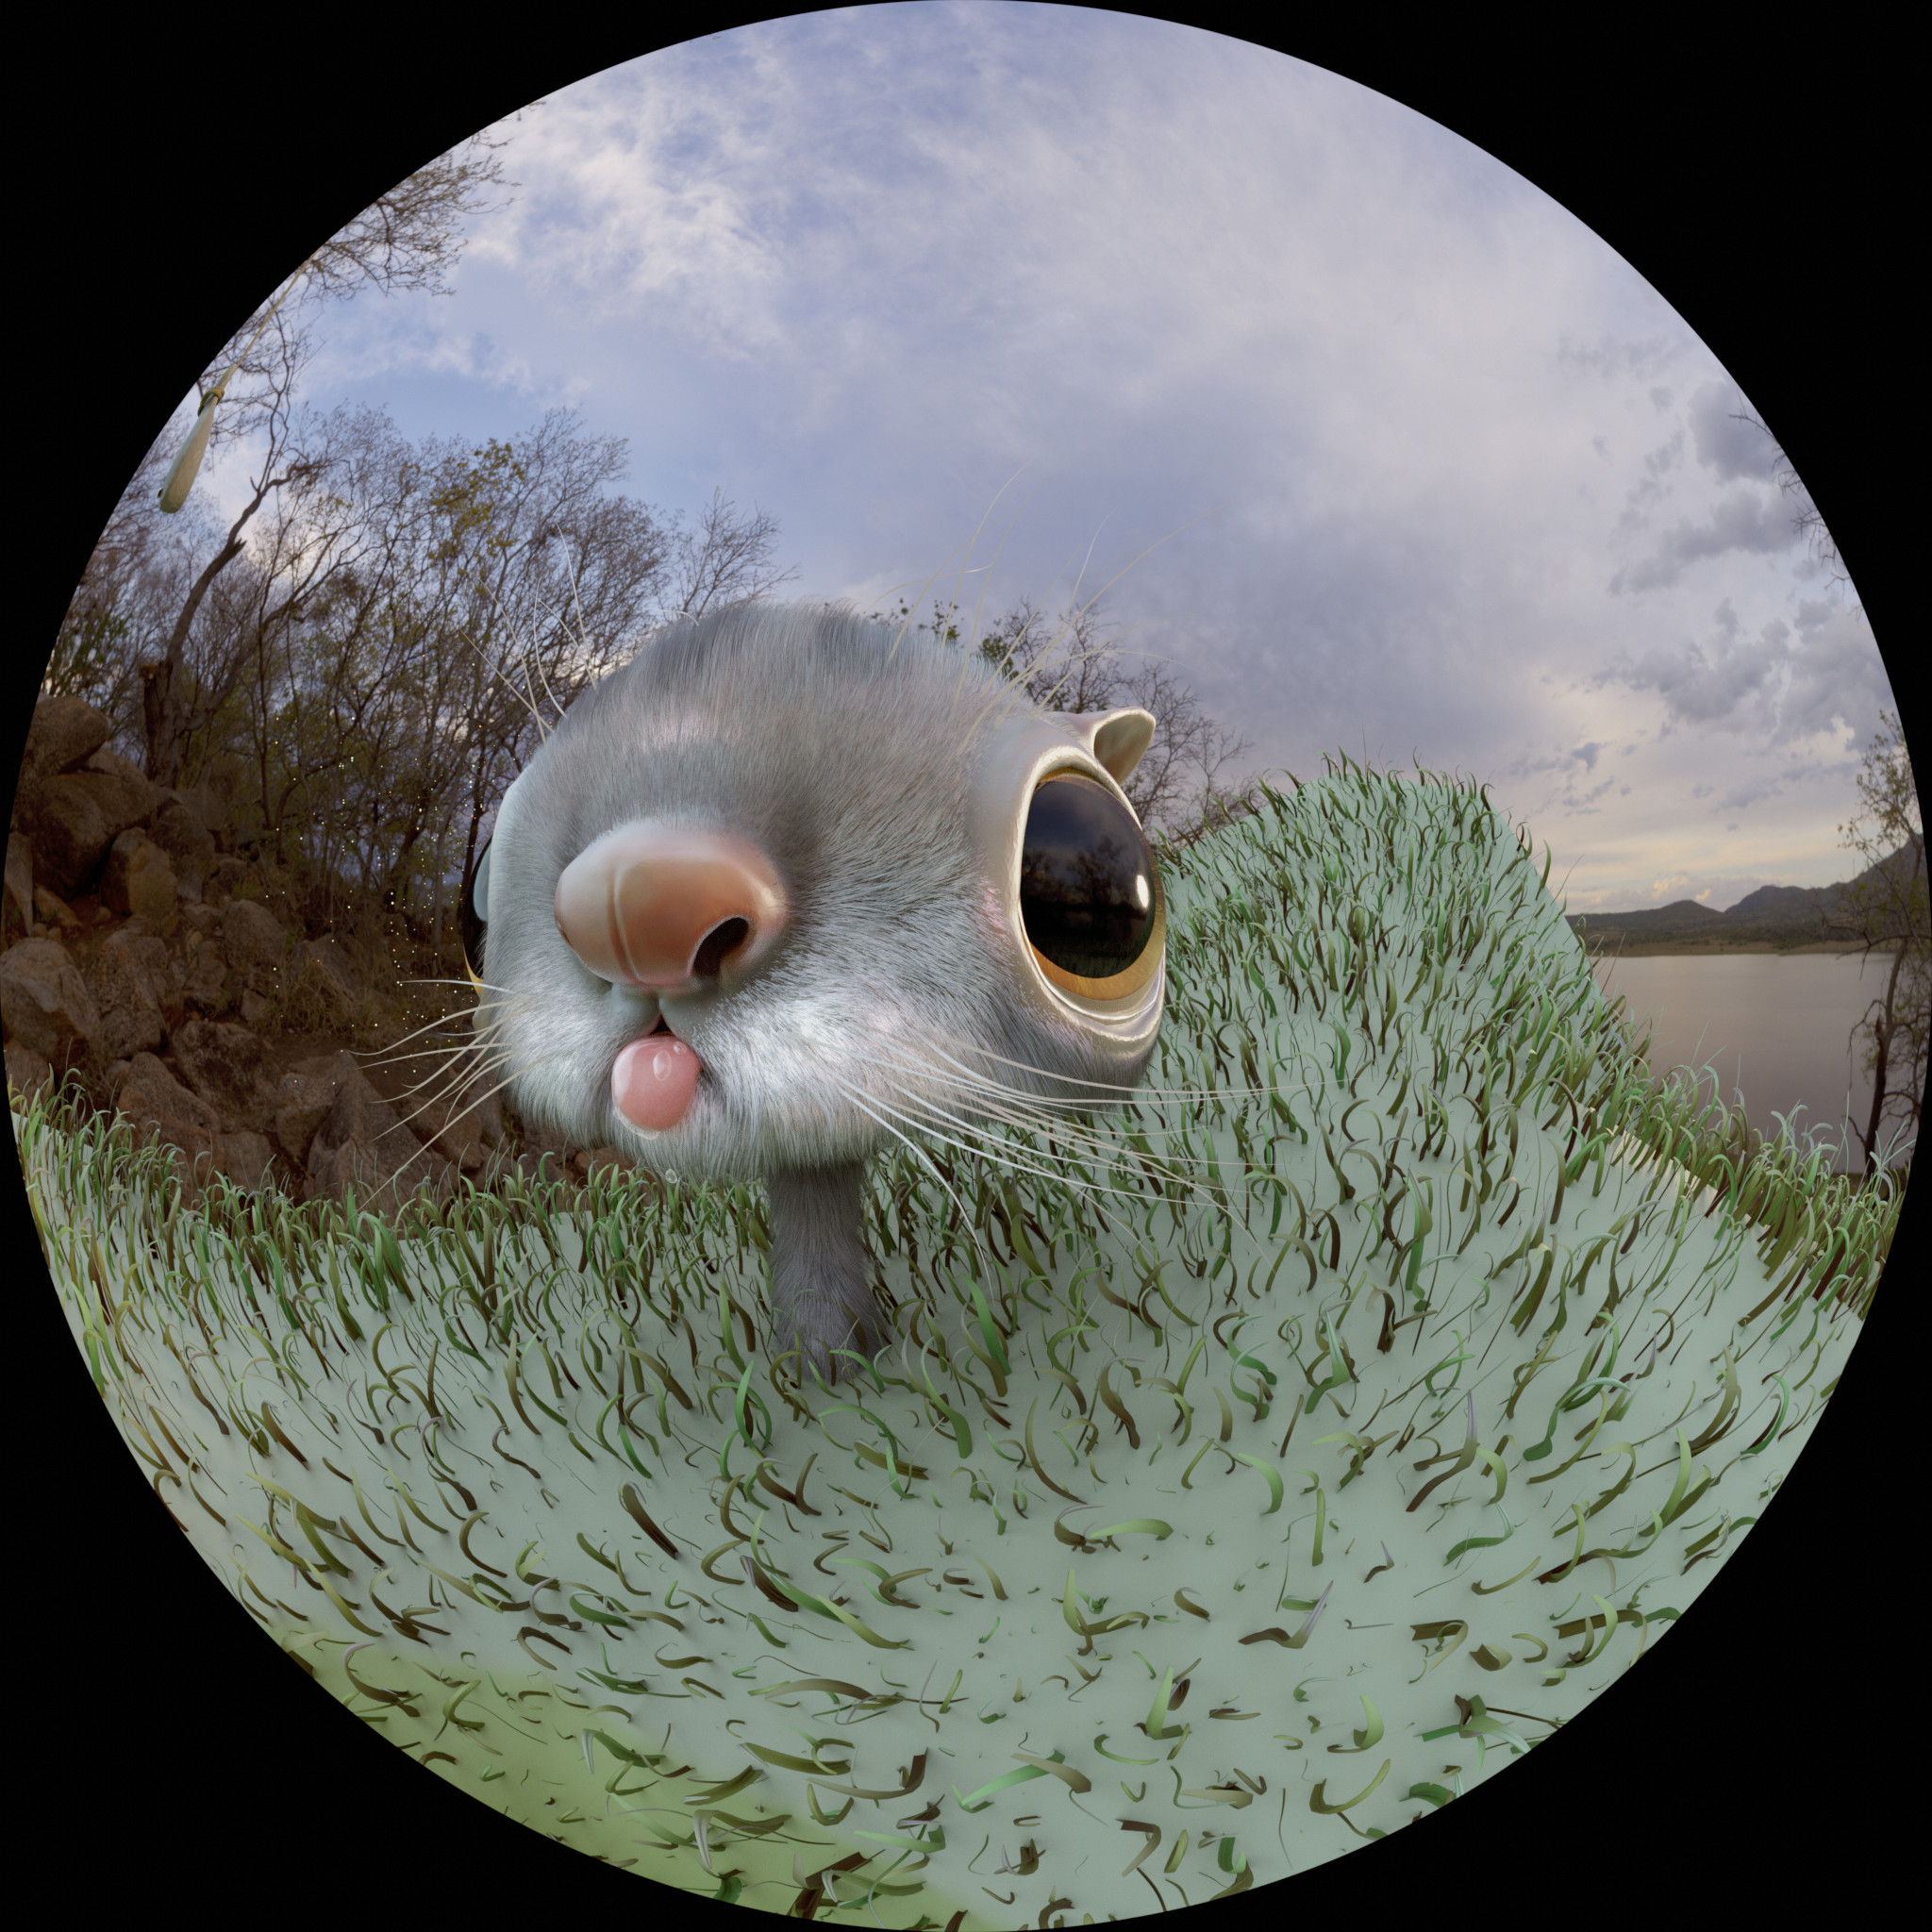
\includegraphics[width=0.25\textwidth]{0001.png}
	\caption{Fisheye image with \ang{190} field of view.}
\end{wrapfigure}
Let \begin{math}
    p = \begin{bmatrix}
		 	p.x & p.y &1
		\end{bmatrix}^{T}
\end{math} be a rectilinear image point. Then by [4], 
\begin{center}
    $P = R^{-1} K^{-1} p$\\
    $r = \|P\|$\\
    $\theta = \arccos(P.z / r)$\\
    $\phi = \arctan2(P.y / P.x)$\\
\end{center}

Using $F$ and $\theta$ in \textit{Equidistant} projection equation above, $r_{d}$ is found and consequently the corresponding fisheye image point $(p'.x, p'.y)$ is determined as below:
\begin{center}
    $r_{d} = F\theta$\\
    $p'.x = r_{d}\cos(\phi) + 0.5 \cdot w$ ($w$ is width of fisheye image)\\
    $p'.y = r_{d}\sin(\phi) + 0.5 \cdot h$ ($h$ is height of fisheye image)\\
\end{center}
There area many interpolation methods (e.g linear, bilinear, cubic, bicubic etc.). Choosing any of them depends on wished quality of the final image. Increasing the quality decreases the speed of the overall program and vice versa. Since bilinear interpolation produces good enough quality with sufficient speed, it is used in PaNaRuf to colour each pixel in the rectilinear image.\\~\\
Applying the above operations, multiple rectilinear images are derived from a single fisheye image. If there are $n$ fisheye images and $m$ rectilinear images are obtained from each of them, then every set of $m$ rectilinear images (along with corresponding camera parameters: K, R matrices) are stored in set $S$ as below:
\begin{center}
$S = \{\{P_{11},P_{12},....P_{1m}\}, \{P_{21},P_{22},....P_{2m}\} ,....\{P_{n1},P_{n2},....P_{nm}\}\}$
\end{center}
Above, each $P_{ij}$ is a tuple of $(I_{ij}, K_{ij} , R_{ij})$ where $I_{ij}$ is j-th rectilinear image obtained from i-th fisheye image, $K_{ij}$ and $R_{ij}$ are its corresponding camera parameters. So, all together,  set of sets $S$ is defined.\\~\\
\begin{figure}[!hb]
\centering
\begin{tabular}{c c c c}
\includegraphics[width = 0.25\textwidth]{1.png}&
\includegraphics[width = 0.25\textwidth]{2.png}&
\includegraphics[width = 0.25\textwidth]{3.png}&
\includegraphics[width = 0.25\textwidth]{4.png}\\
\includegraphics[width = 0.25\textwidth]{5.png}&
\includegraphics[width = 0.25\textwidth]{6.png}&
\includegraphics[width = 0.25\textwidth]{7.png}&
\includegraphics[width = 0.25\textwidth]{8.png}
\end{tabular}
	\caption{Acquired 8 rectilinear images by rotating virtual pinhole camera after un-projecting the fisheye (Figure 1) image points to 3D unit sphere.}
\end{figure}
\section*{Find relations among image sets}
The image orientations, within the same set, relative to each other, are clear because their corresponding camera parameters (R,K) are known. However, an orientation between any two images, each of which belongs to different sets in $S$, is undefined. This section concentrates mainly on estimating such orientations so as to find relations among each possible image sets.

If there is a relation between any two image sets in $S$, it can only be understood by checking whether there exist an image in one set well-overlapping with an image in the other set or not.  In order to find such a good overlap between any two images, first of all, their matching 2D points are obtained as described in the next sub-section.\\~\\
\textbf{A. Extract features:}
Thanks to OpenCV, SIFT and BestOf2NearestMatcher properties are used to estimate the matching points between any two images. Using SIFT (Scale-Invariant Feature Transform), the features of the images are extracted. Then, match distances ratio threshold is chosen as 0.65 and BestOf2NearestMatcher is applied to estimate matched points between two images. 

It is assumed that the matching points between two images are estimated. Then, the next step is to estimate the homography matrix (or pojective transformation matrix) $H$  between these images. The main reason why it should be computed is that it is a way for finding relation between these images  each of which is a member of two different sets. If this relation is created then the orientations among the all images in two image sets, reletive to each other can be established.

The basic algorithm of computing homography matrix $H$ is Direct Linear Transform algorithm. However, in practice, it is possible to have bad matches. To ensure that the estimated homography is acceptable, DLT algorithm is used with RANSAC (Random Sample and Consensus algorithm). Then it becomes RANSAC-based homography estimation algorithm. Before explaining this algorithm, the DLT algorithm should be introduced first.\\~\\
\textbf{B. Direct Linear Transform:} Let $p$ be 2D point of first image and $p'$ be 2D point of second image in homogeneous coordinates, such that $H$ projectively transforms $p$ to $p'$. Then, the general equation becomes as:
\begin{center}
	$ \alpha \cdot p' = H\cdot p$
\end{center}
where $\alpha$ is a non-zero scale factor.\\
The equation above can also be written in the form of $p' \times Hp = 0$ ($\alpha$ is reduced due to equality with zero) and consequently the set of equations $Ah = 0$ can be derived as[7]: 
\begin{equation*}
    Ah = \begin{bmatrix}
			0 & 0 & 0 &-p.x &-p.y &-1 &p'.y \cdot p.x & &p'.y \cdot p.y &p'.y\\
			p.x & p.y & 1 &0 &0 &0 &-p'.x \cdot p.x & &-p'.x \cdot p.y &-p'.x
			\end{bmatrix} \cdot \begin{bmatrix}
			h_{1}\\
			.\\
			.\\
			.\\
			h_{9}
			\end{bmatrix} = 0 
\end{equation*}
where  $h$ is the vector of unknown entries of $H$, and $A$ is a 9 x 2 matrix. Since there are 9 unknowns and 2 equations, the above operations are applied to 3 more point correspondences. Thus, $A$ becomes  a 9 x 8 matrix. Using $UDV^{T} = A$ (singular value decomposition), and by taking the last row of $V^{T}$, $h$ is computed and 3 x 3 homography matrix $H$ is constructed from $h$. Finally, $H$ is normalized by dividing all elements by $H_{33}$.\\~\\
This is the primitive DLT algorithm that is explained above. However, according to Hartley and Zisserman in [7], a normalization step should be added to DLT algorithm to have more accurate $H$.
Then, the common apporach for accurate DLT algorithm becomes as below:
\begin{enumerate}
\item Take matching 4 point correspondences in homogeneous coordinates: $p_{i}$ and $p'_{i}$ where $p'_{i} = Hp_{i}$ and $i$ represents the index of these point correspondences.
\item Find a 3 x 3  matrices $T$, $T'$ that respectively translates and scales the centroid of points $p_{i}$ and $p'_{i}$ to the origin so that their average distance from origin becomes $\sqrt{2}$.
\item Use DLT and compute homography matrix $H$ taking the transformed point correspondences.
\item Reset $H$ by $H = T'^{-1} H T$
\end{enumerate}
\ \\~\\
\textbf{C. RANSAC-based homography estimation:}
The homography estimation is based on Random Sample Consensus (RANSAC) since it is the most widely used robust estimation method, as indicated in [6]. The main algorithm for RANSAC-based homography estimation is explained below:
\begin{enumerate}
\item Set $p = 0.99$ based on [7], and $N = 1000$. Start iteration from 1 to N
\item At each iteration, randomly choose 4 correspondences from matched points.
	\begin{itemize}
		\item If any 3 points are on the same line (colinearity), do nothing and continue to iteration.[7]
		\item If there exist repeated point among them, do nothing and continue to iteration.
	\end{itemize}
\item Use these points in DLT algorithm defined above, to estimate homography H.
\item Check all matching 2D points in homogeneous coordinates with estimated homography H and classify them as inlier or outlier based on their concurrence with H.
	\begin{itemize}
		\item Inlier if $ d < t$
		\item Outlier if $ d \geq t$
	\end{itemize}
where $d$ is error acquired from both forward and backward transformation applied by H. $t$ is distance threshold such that $ t = \sqrt{5.99} \cdot \sigma$ where $\sigma$ is standard deviation [7]. 
\item If better H  is estimated with more inliers, do the following:
\begin{itemize}
		\item update homography with the current H.
		\item update the number of inliers
		\item update $N$ by $N = \log(1-p) / \log(1-(1-\epsilon)^{4})$ where $\epsilon = 1-w$, such that $w$ is the probability that any data point is an inlier [7]. 
	\end{itemize}
\item After the iteration is over, re-estimate the homography (via DLT) using the matching points that are inliers [7].
\end{enumerate}
\ \\~\\
\textbf{D. Update appropriate rotation matrices:}
If a homography matrix is estimated between two images each of which belongs to different sets in $S$, then the relation between these sets is established as described below with an example.

$I_{1i}$ is assumed to overlap with $I_{2j}$ where $i,j = 1,...,m$. It is also assumed that the images in the second set should be aligned to the images in the first set. Then, the following operations are applied to find the relative rotation matrix $R_{rel}$. 
\begin{center}
    $H = K_{1i}R_{1i}R^{-1}K^{-1}_{2j}$ \\   
    $R = K^{-1}_{2j}H^{-1}K_{1i}R_{1i}$ \\
    $R_{rel} = R^{-1}_{2j}R$\\
\end{center}
Then, the whole rotation matrices in second set are updated by simply multiplying them with the relative rotation matrix $R_{rel}$ as below:
\begin{center}
    $R_{2k} = R_{2k} \cdot R_{rel}$ where $ k = 1,...m$\\
\end{center}
Using the whole operations described in the current section, all possible relations among the image sets are estimated. Thus, the orientations of the whole images, relative to each other, are known, no matter if they are in the same set or not.\\~\\
Now, every parameter in the software is clear: the images, their corresponding rotation and calibration matrices, the orientations among them. Using these parameters, spherical mapping operation is applied to each rectilinear image to acquire spherical warped image from each of them.\\~\\
\section*{Equirectangular/Spherical Warping:}
In this section, a spherical mapped image is obtained from each rectilinear image separately. These mapped images, all together, creates spherical panoramic image by getting stittched. The first step to convert a rectilinear image to a sphercial warped image is forward spherical mapping operation that is applied to each 2D points of the rectilinear image in homogeneous coordinates. This is important because the destination/spherical image size (width and height) should be identified.\\~\\
\textbf{A. Forward Mapping:}
 Let \begin{math}
    p = \begin{bmatrix}
		 	p.x\\
		    p.y\\
             1
		\end{bmatrix}
\end{math} be a rectilinear image point. Then, the whole forward warping operation for point $p$ is described as below:\\~\\
\textit{2D to 3D world[2]:}
\begin{center}
	 $P = R^{-1}  K^{-1} p$ 
\end{center}
\textit{3D world to 3D unit-sphere [8]:}
\begin{center}
	 $C = \frac{P}{\sqrt{P.x^{2} + P.y^{2} + P.z^{2}}}$
\end{center}
\textit{3D unit-sphere to spherical coordinates $(\theta, \phi)$ [8]:}
\begin{center}
	 $\theta = \arctan2( C.x, C.z)$\\ 
	 $\phi = \arctan2(C.y, \sqrt{C.x^{2} + C.z^{2}})$
\end{center}
\textit{Spherical coordinates to spherical warped image coordinates [8]:}
\begin{center}
 	 $x_{sph} = \theta \cdot f$ \\
	 $y_{sph} = \phi \cdot f$  
\end{center}
This forward mapping operation is applied to all points of each rectilinear image to find the size of the spherical warped image. The size is calculated by taking minimum and maximum of $(x_{sph}, y_{sph})$. Then, the minimum/top-left/tl and maximum/bottom-right/br points are used to find the width and height of the spherical warped image.
\begin{center}				
				$width = br.x - tl.x$ \\ 
				$height = br.y - tl.y$
\end{center}
Thus, the destination image size is determined by using the above operations. \\~\\
\textbf{B. Backward Mapping:}
In this sub-section, spherical warped image and corresponding mask are declared with the determined image size and the folowing operations (reverse of the forward mapping operations) are applied to each spherical warped image point to get the corresponding rectilinear image point $p$.
\begin{center}
$\theta = \frac{x_{sph}}{f}$\\~\\
$\phi = \frac{y_{sph}}{f}$\\~\\
$C.x = \sin(\theta)\cos(\phi)$\\~\\
$C.y = \sin(\phi)$\\~\\
$C.z = \cos(\theta)\cos(\phi)$\\~\\
$P = \frac{C}{|C.z|}$\\~\\
$p = K \cdot R \cdot P$\\~\\
$p = \frac{p}{p.z}$
\end{center}
Then, using the pixel value of corresponding point $p$, the spherical warped image point  $(x_{sph}, y_{sph})$ is coloured. Again, bilinear interpolation method is used for this. The spherical warped mask , on the other hand, keeps track of the points $(x_{sph}, y_{sph})$ when corresponding point $p$ is outside of the rectilinear image.\\
So, applying the spherical mapping operations to each rectilinear images, the corresponding spherical warped images along with their sizes, top-left corners and the spherical warped masks are stored for getting used in the next stittching section.\\~\\
\section*{Stittching:}
In this section, the software uses two properties (GraphCutSeamFinder and Multi-band blending) of OpenCV to stittch the spherical warped images. Firstly, using spherical warped images and masks, the
GraphCutSeamFinder estimates the seams. Then, Multi-band blending uses their sizes and top-left corners to stittch and blend them. Finally, a spherical image with field of view 2 : 1-ratio (360 degrees horizontal, 180 degrees vertical), is obtained. \\~\\
\section*{Evaluation:}
The whole procedure that the software applies to acquire a spherical panoramic image from multiple overlapping fisheye images, was explained in the previous sections step-by-step. Now, in this section, 
some input well-overlapping fisheye images, and their results achieved by the software are displayed. Then, the success/failures of the software is discussed based on the results.\\~\\
\begin{figure}[h!]
  \centering
  \begin{subfigure}[b]{0.2\linewidth}
    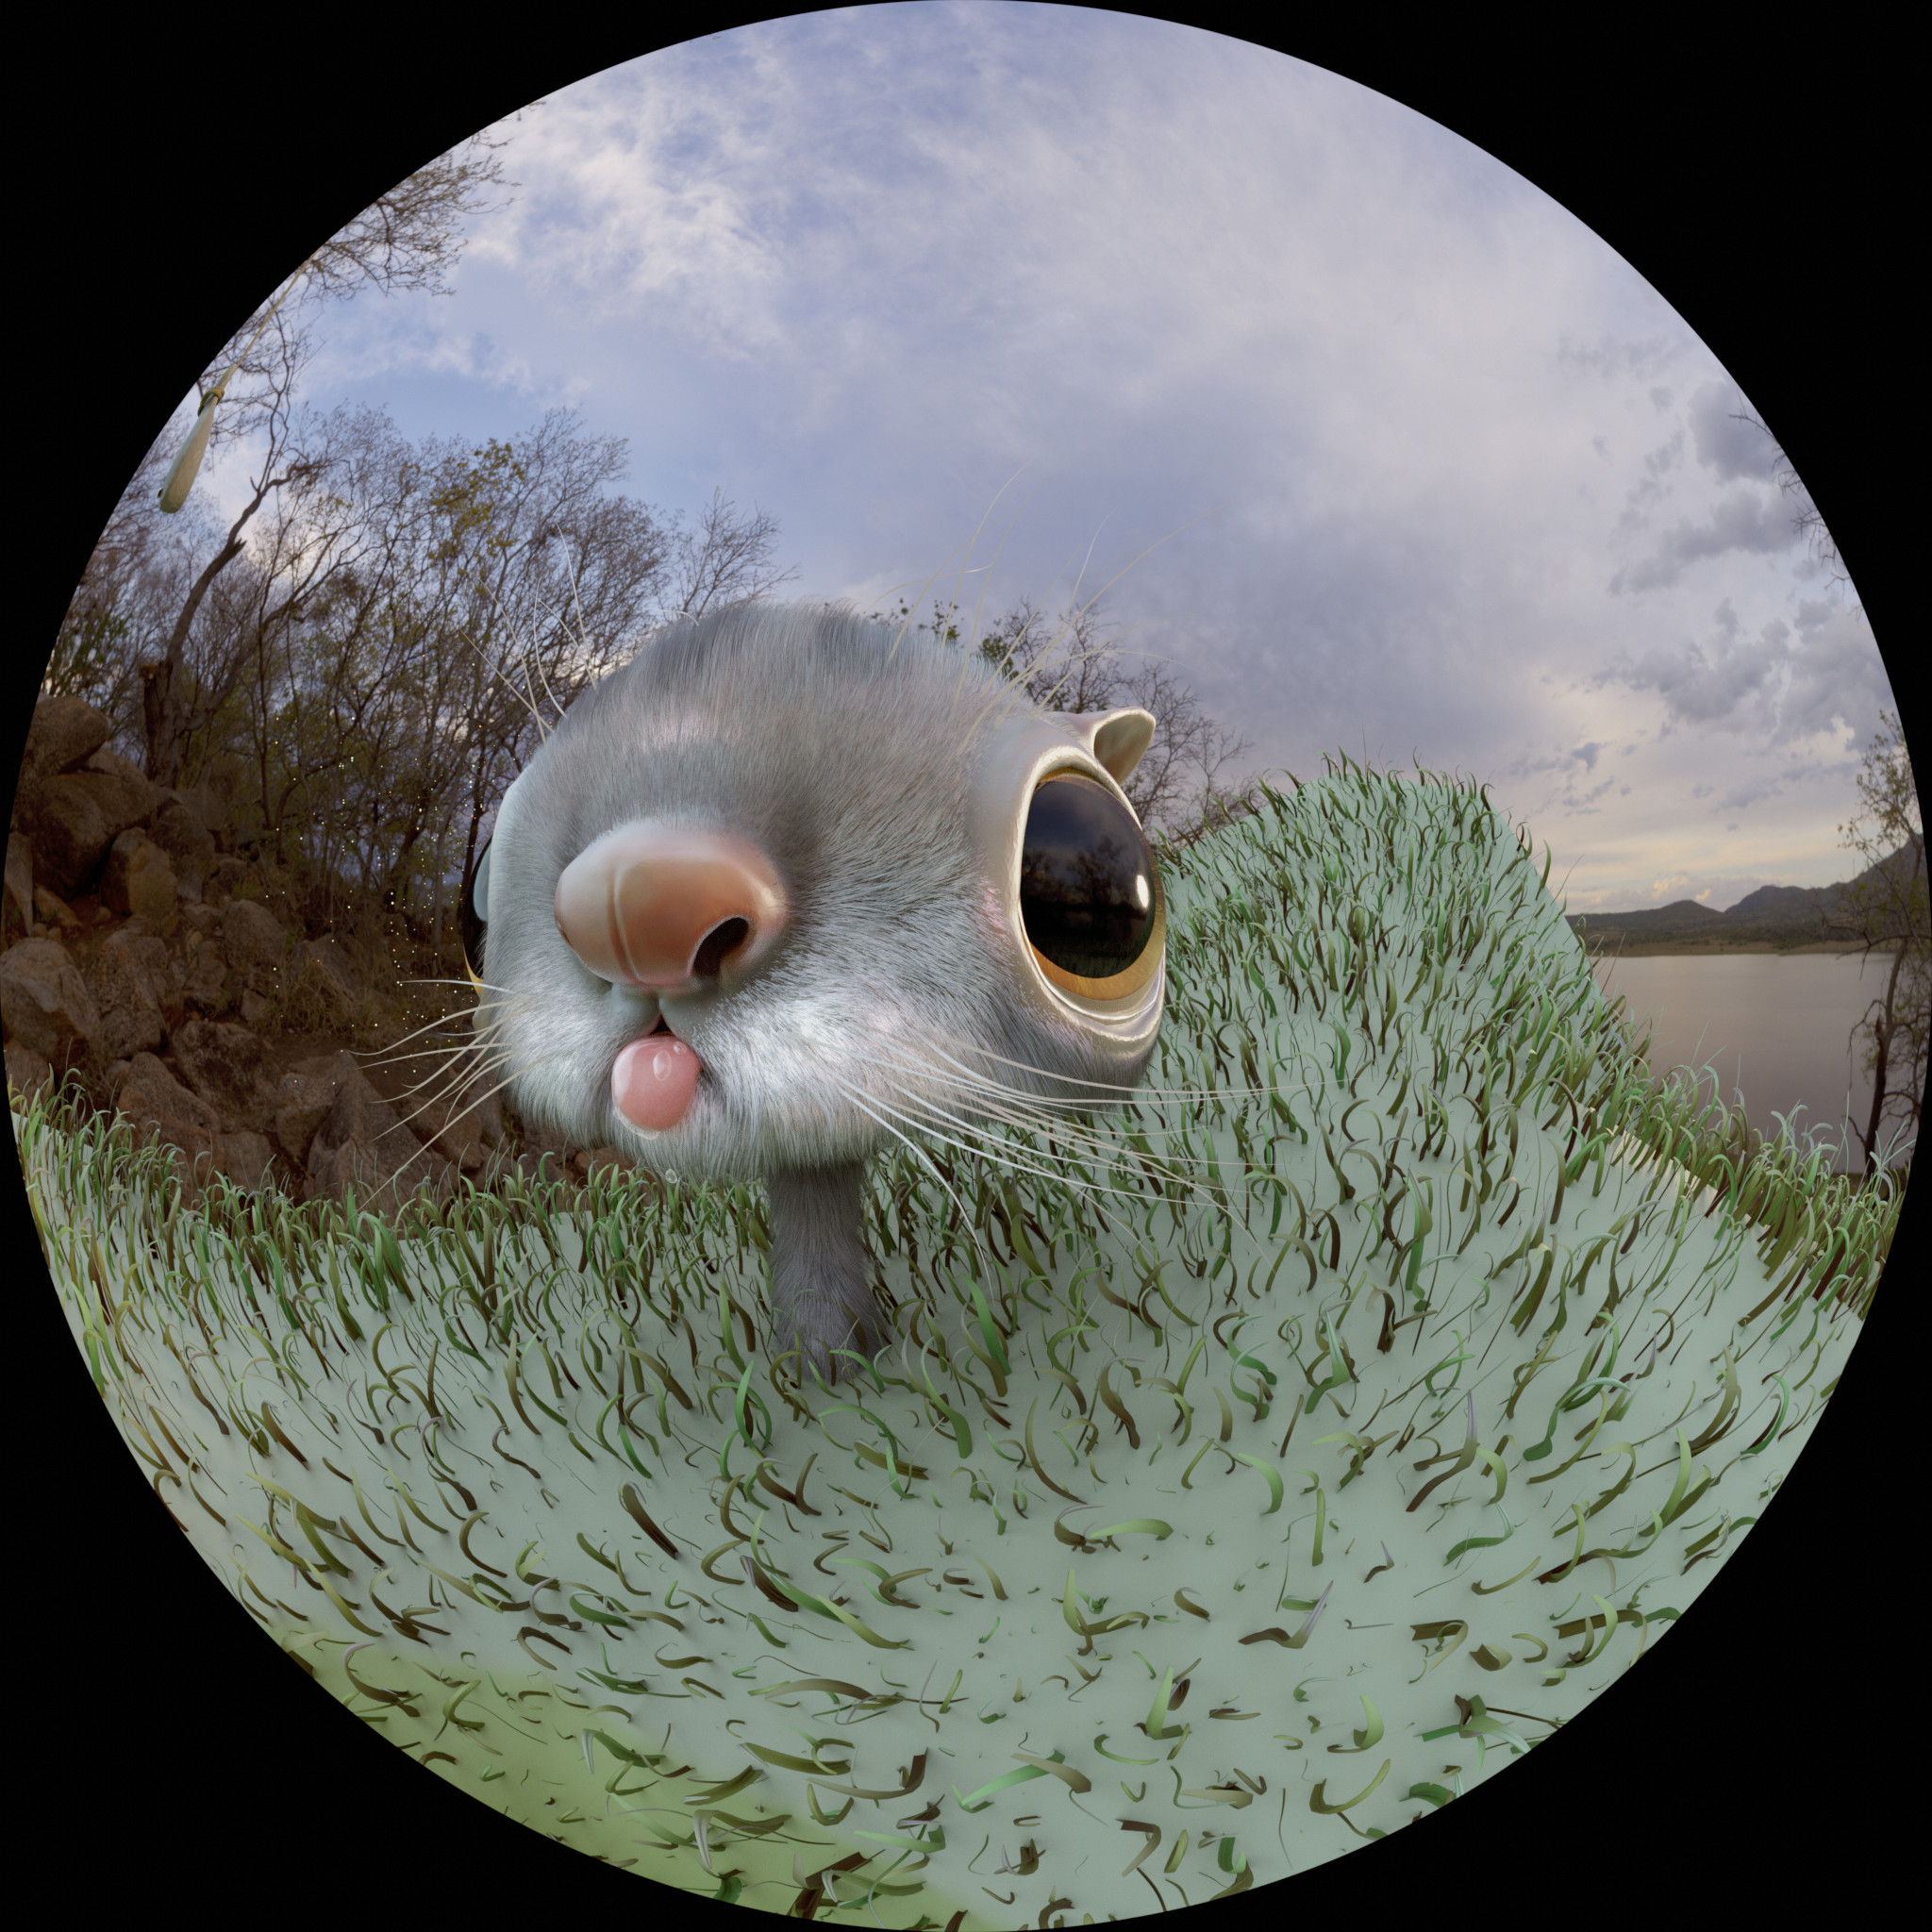
\includegraphics[width=\linewidth]{0001.png}
  \end{subfigure}
  \begin{subfigure}[b]{0.2\linewidth}
    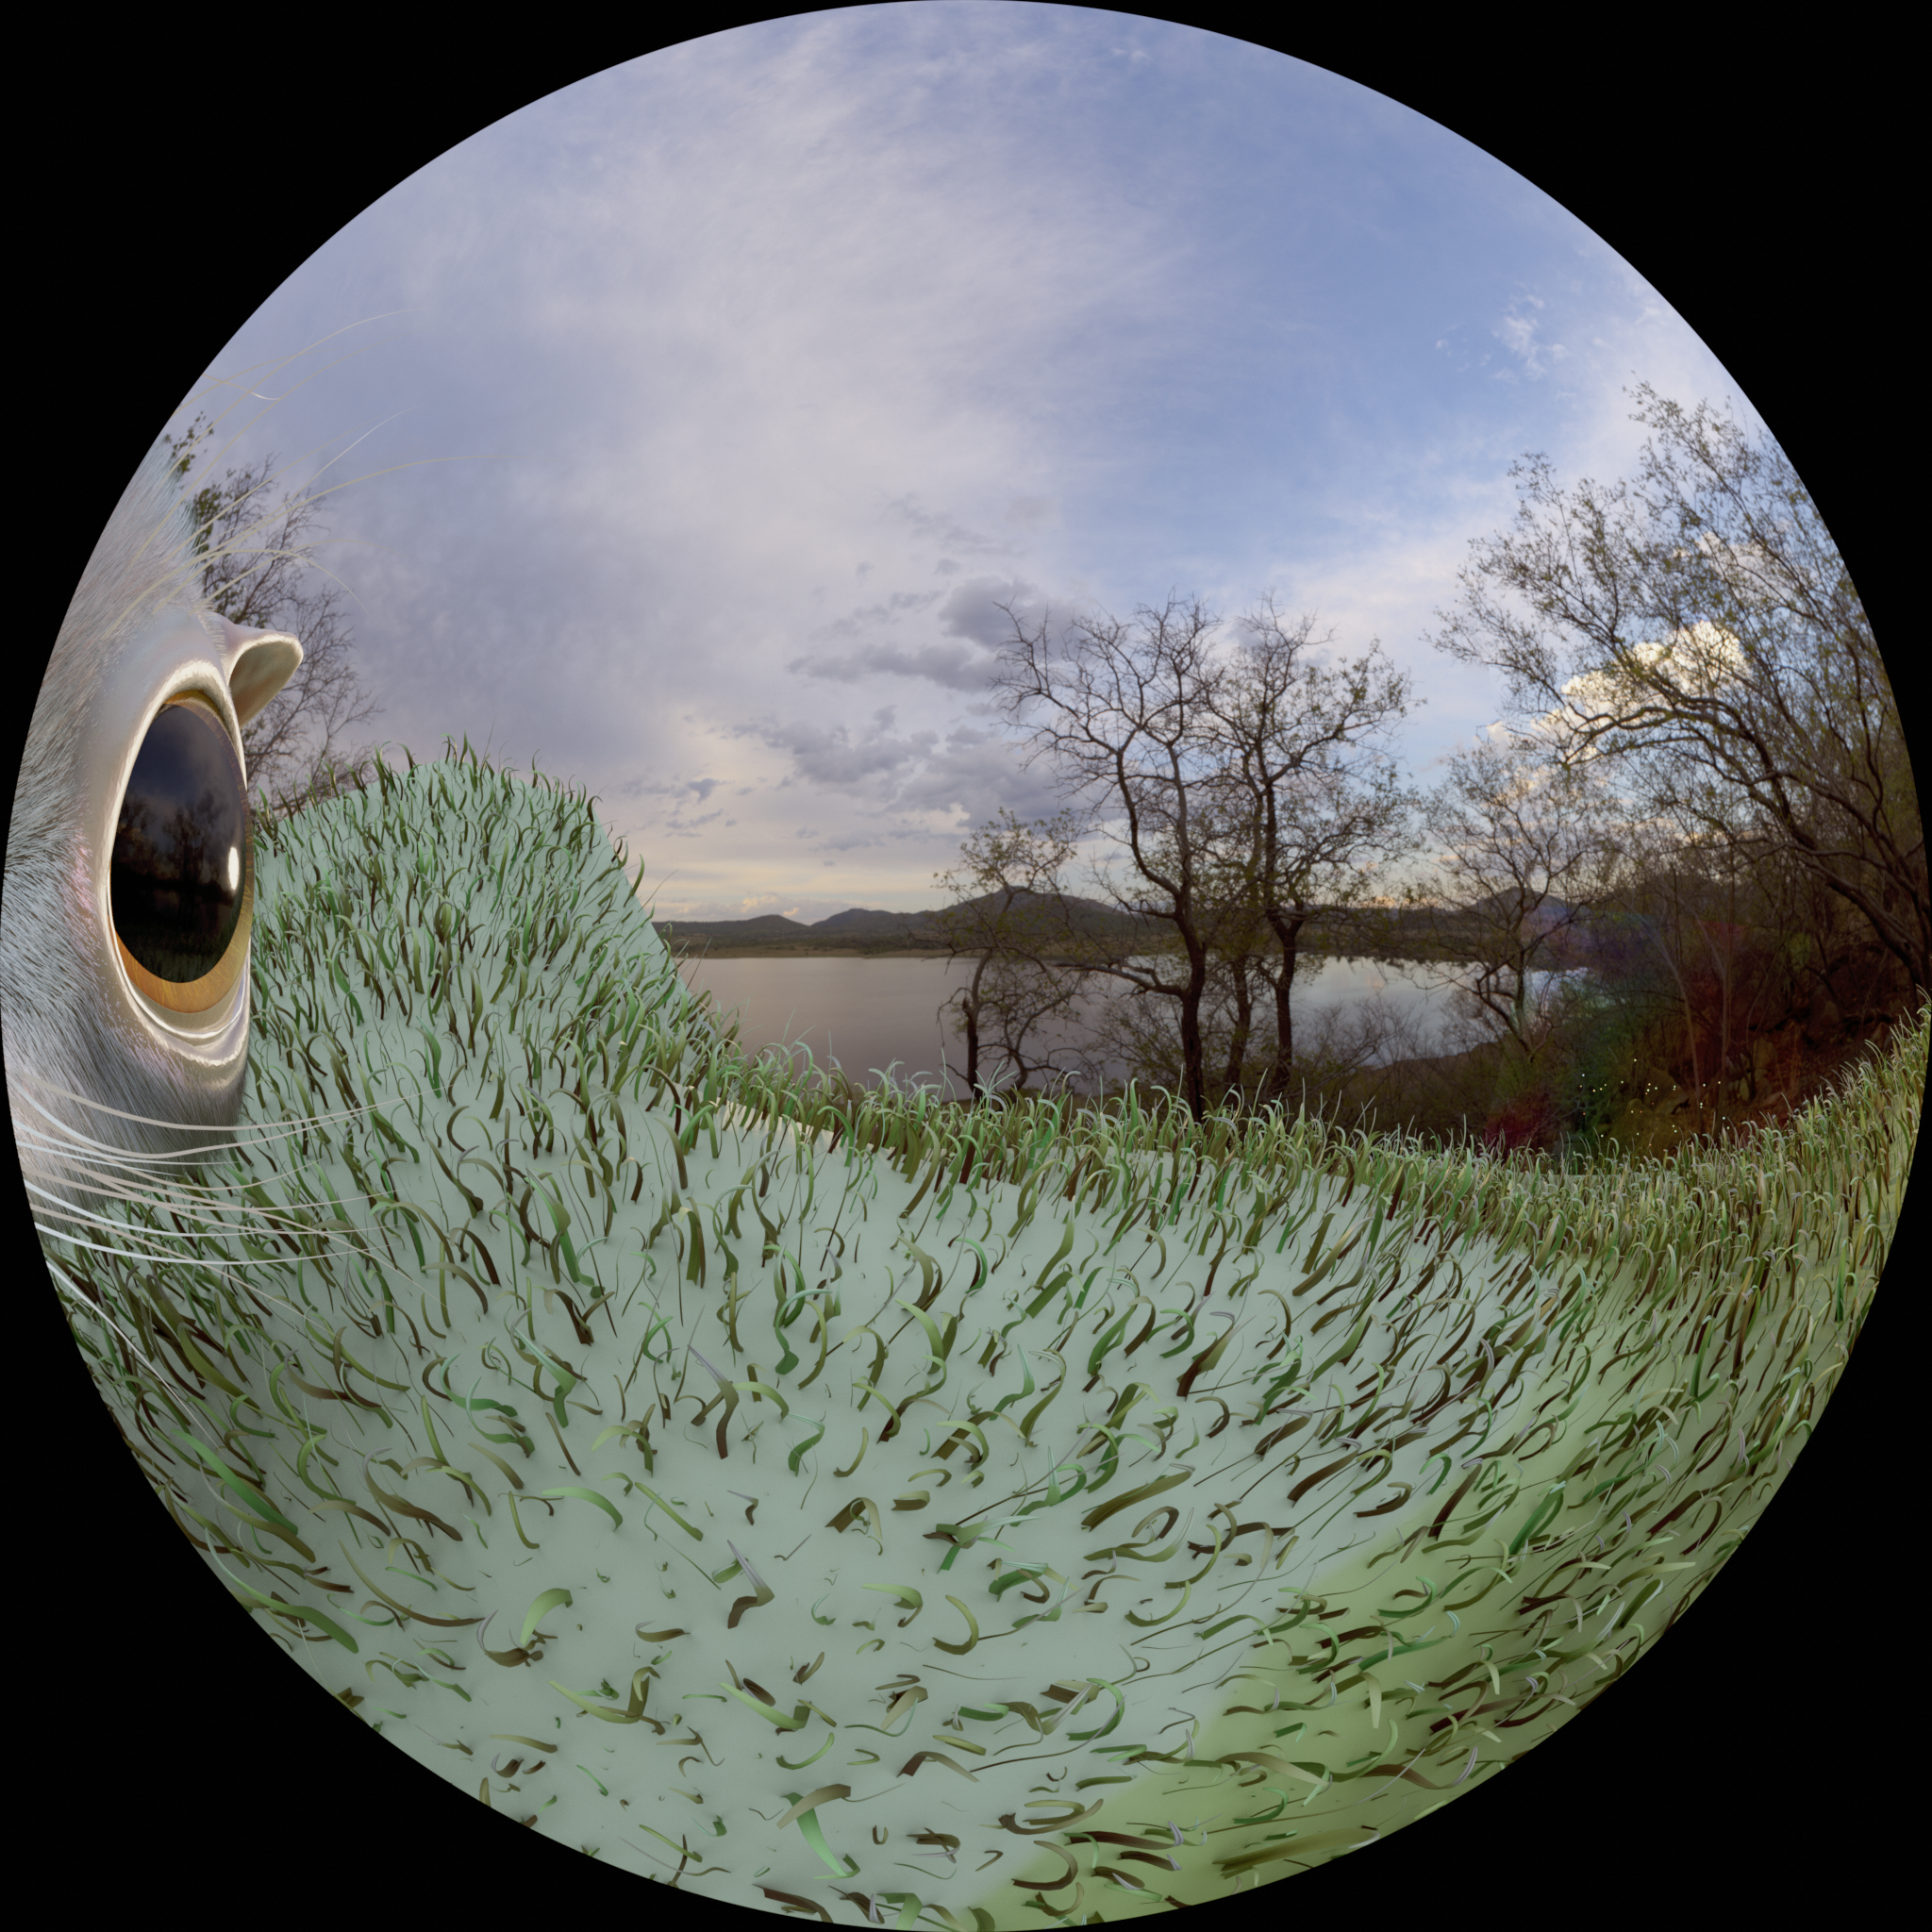
\includegraphics[width=\linewidth]{0002.png}
  \end{subfigure}
  \begin{subfigure}[b]{0.2\linewidth}
    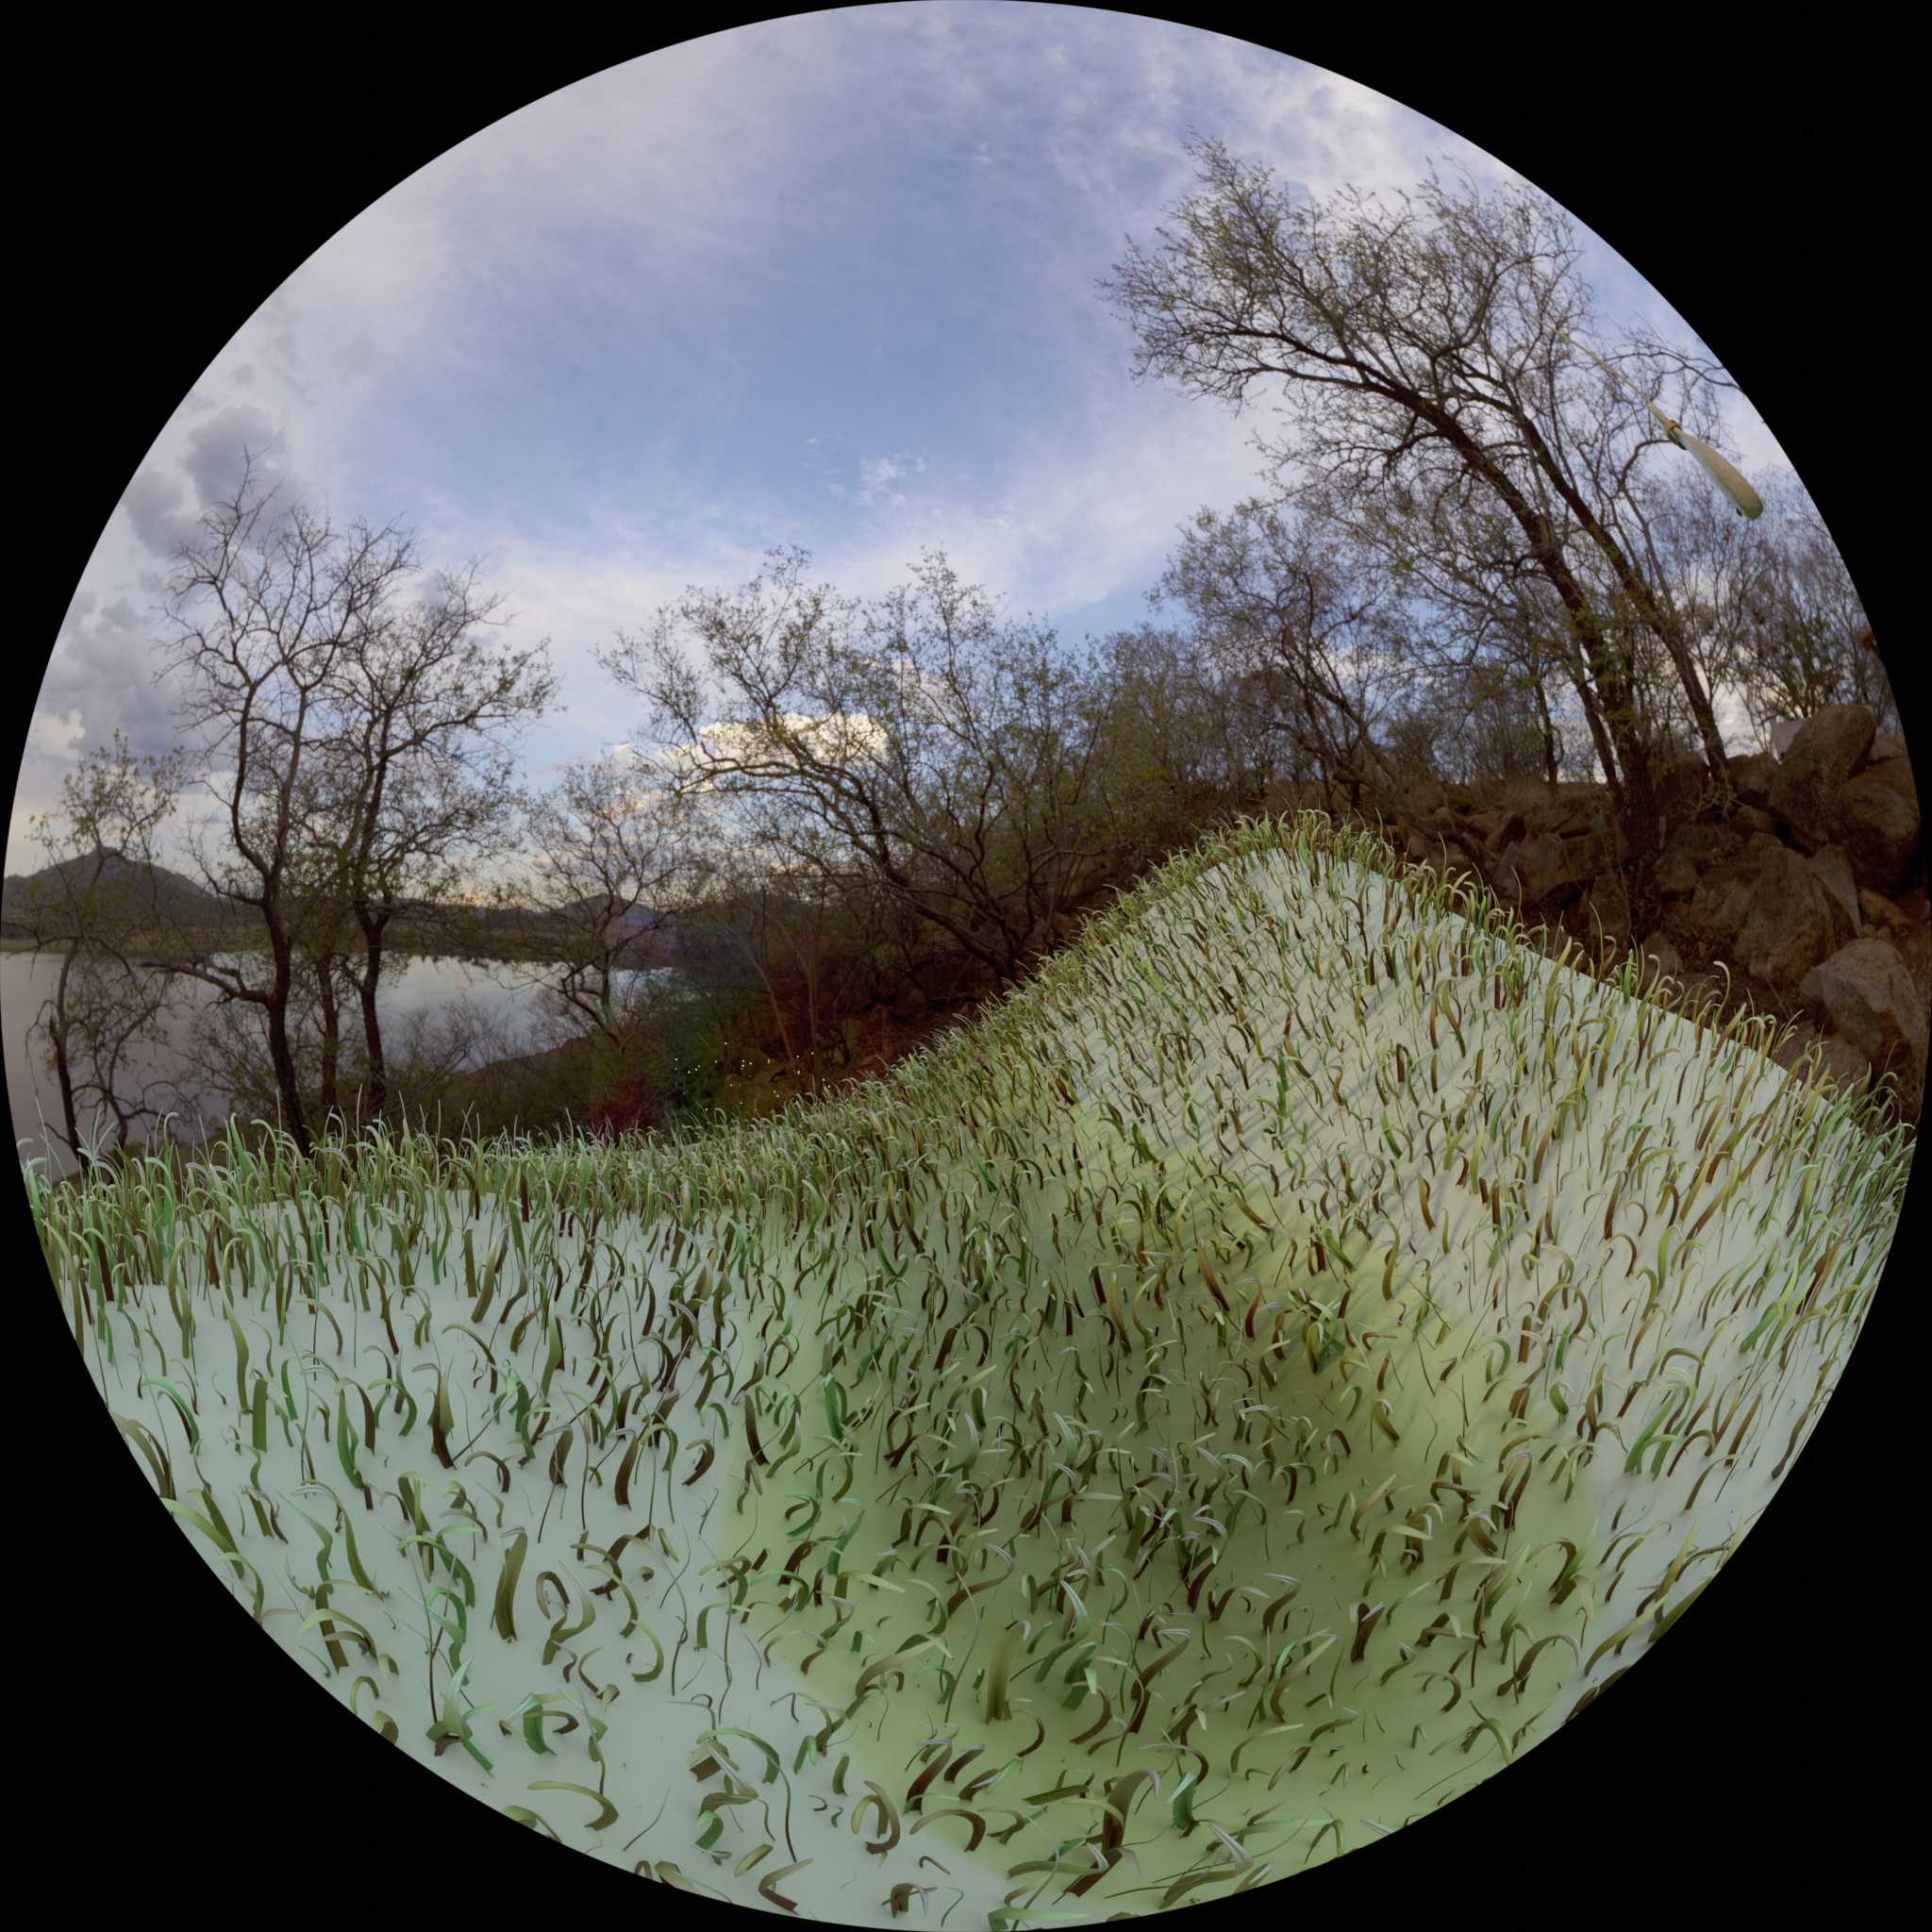
\includegraphics[width=\linewidth]{0003.png}
  \end{subfigure}
  \begin{subfigure}[b]{0.2\linewidth}
    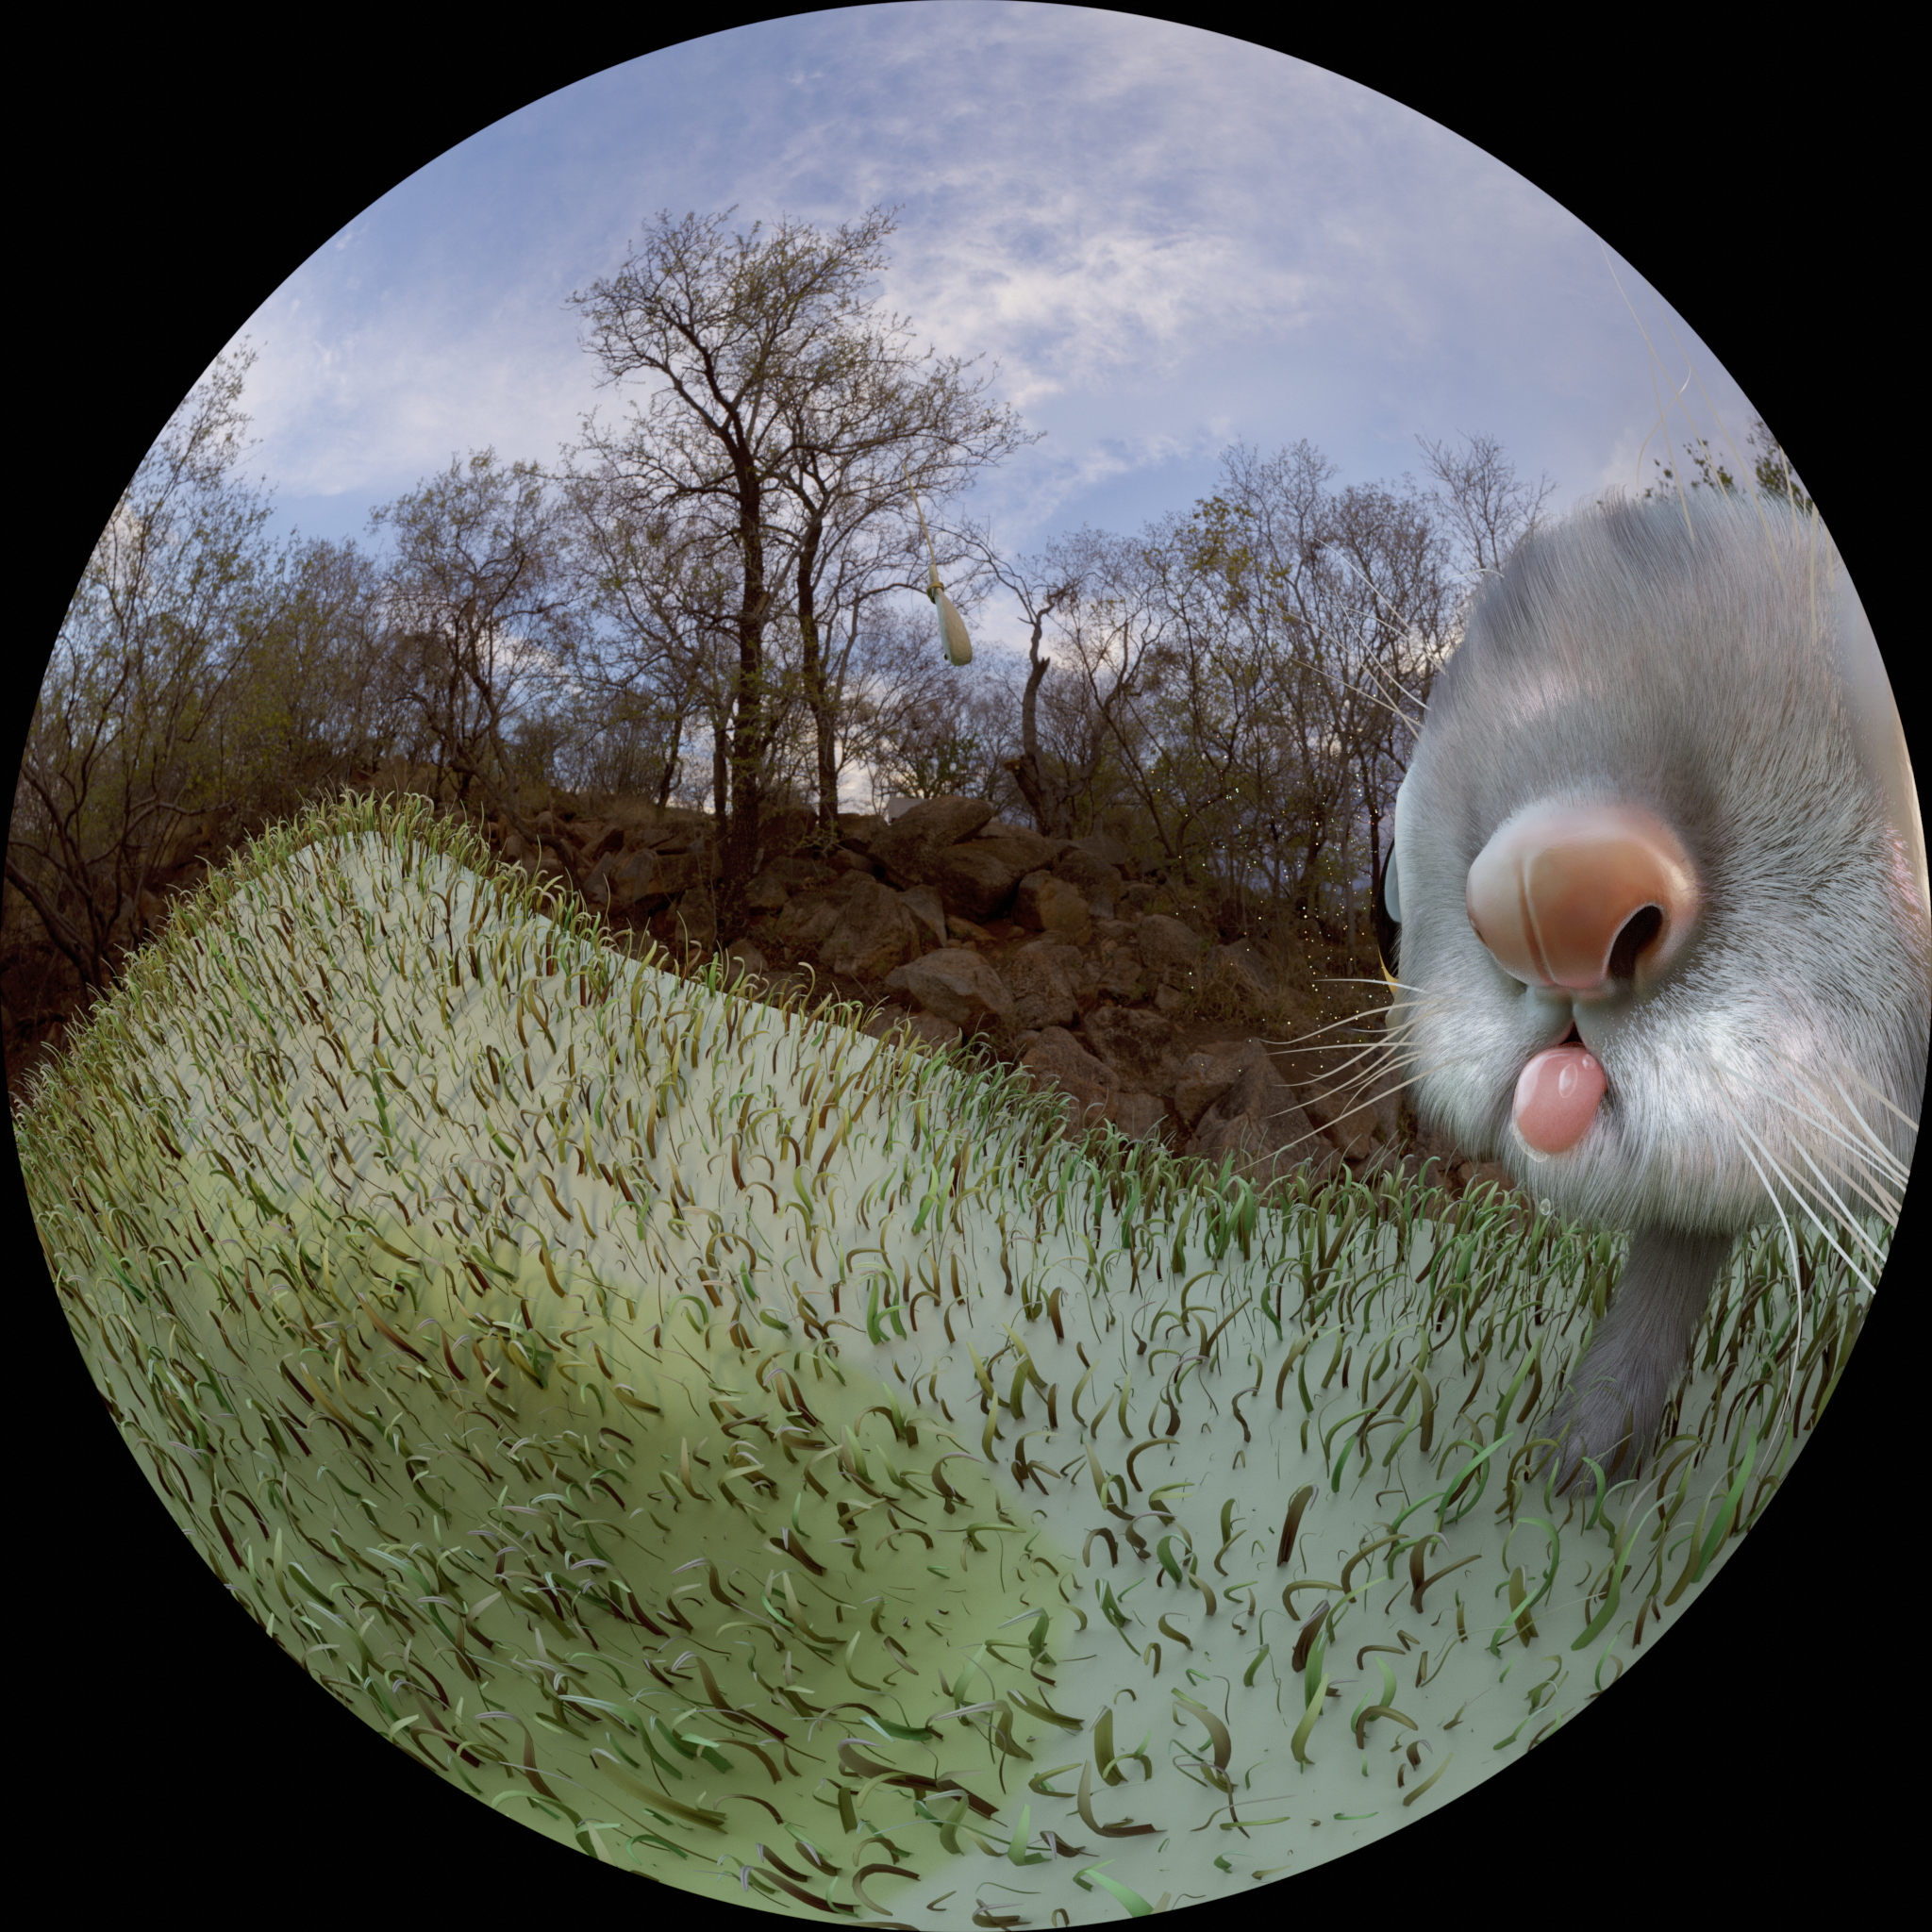
\includegraphics[width=\linewidth]{0004.png}
  \end{subfigure}
    \caption{52.6\%-overlapping fisheye images with \ang{190} FOV.}
  \begin{subfigure}[b]{1.0\linewidth}
    \includegraphics[width=\linewidth]{rabbit.png}
  \end{subfigure}
  \caption{Spherical panoramic 864 x 432 image result with PaNaRuf.}
\end{figure}
\ \\~\\
\textit{Quality:}
The Figure 3 displays four overlapping fisheye images, each with 190 degrees field of view, and the Figure 4 shows the result that has been achieved by the software. The result is good enough and it holds the $2 : 1$ -ratio property of spherical panorama, but its quality is not as perfect as desired. There are two main reasons of such quality.

The first reason is that every rectilinear image size (300 x 300) is chosen by default. This is done for speeding up the program. Increasing the number of pixel by size will increase the quality as well but will decrease the overall run time of the program.

The second reason is the interpolation method chosen. In both mapping physical fisheye image to rectilinear image and spherical warping operations, bilinear interpolation method is used for coloring each pixel.  However, as it was mentioned in the previous sections, choosing better interpolation method will increase the quality but will decrease, again, the speed of the software.\\~\\
\begin{figure}[h!]
  \centering
  \begin{subfigure}[b]{0.2\linewidth}
    \includegraphics[width=\linewidth]{1.jpg}
  \end{subfigure}
  \begin{subfigure}[b]{0.2\linewidth}
    \includegraphics[width=\linewidth]{2.jpg}
  \end{subfigure}
  \begin{subfigure}[b]{0.2\linewidth}
    \includegraphics[width=\linewidth]{3.jpg}
  \end{subfigure}
  \begin{subfigure}[b]{0.2\linewidth}
    \includegraphics[width=\linewidth]{4.jpg}
  \end{subfigure}
    \caption{50\%-overlapping fisheye images with \ang{180} FOV.}
  \begin{subfigure}[b]{1.0\linewidth}
    \includegraphics[width=\linewidth]{result.png}
  \end{subfigure}
  \caption{Spherical panoramic 942 x 471 image result with PaNaRuf.}
\end{figure}
\ \\~\\
\textit{Accuracy:}
The result images sometimes can produce small amount of errors especially around stittching areas among the image sets. For instance, another 4 well-overlapping fisheye images ( in Figure 5.) each with 180 degrees field of view, are used to create a \ang{360} spherical panoramic image (in Figure 6.) using PaNaRuf. In the result of the software, it is obviously seen that there are accuracy errors in top, bottom and left side of the result image. The main reason of such errors is many ''estimations'' applied by the software. To illustrate, estimating relations among image sets or estimating seams among the spherical warped images can produce such accuracy errors since  ''estimation'' does not give $100\%$ guarantee. \\~\\
\textit{Complexity}
The running time of the software for getting a spherical panoramic image from the above inputs (in Figure 3,5) is around 24.17 minutes. This is too much but acceptable because of three main reasons explained below:\\~\\
The first reason is \textit{pixel-wise operations}. In other words, from each fisheye image, 8 rectilinear images are obtained. Since there are 4 fisheye images, there are $8\cdot4 = 32$ rectilinear images in all. Each rectilinear image is acquired by coloring each pixel separately. Similarly, spherical forward and backward mapping operations are applied to each pixel of 32 rectilinear images.\\
The second reason is \textit{finding relations} among image sets. To illustrate, each rectilinear image in one set is checked with all rectilinear images in the other sets for finding possible relationships among the image sets. Thus, many combination of image pairs are searched. \\
The last reason why the program is slow is \textit{finding seams} among 32 rectilinear images. They are waiting for getting stittched but first of all, the program needs to find the seam areas among them. This, all together takes enough time for the software to process.\\~\\
However, applying OpenMP with 8 threads, in pixel-wise operations and finding relations among image sets, reduced the overall run time from 24.17 minutes to 5.32 minutes.\\~\\
\section*{Conclusions and Future perspectives:}
The purpose of this report was to introduce the PaNaRuf which has totally been implemented by me. Firstly,  the need for such a software was discussed in the report. Then, the theory and implementation of it, was explained as a workflow in detail. Finally, the tested images along with the practical success and failures of the results were analyzed. 

For the future, it is planned to add some features to the program for making it produce more accurate and faster results. The implementation of the program is going to be changed based on using graphics processing unit (GPU) instead of central processing unit (CPU) since it has highly parallel structure which helps faster image processing. This modification will definitely result with speeding up the program. With such efficient complexity, it will be possible to apply other updates to the software so as to increase the quality of the result image (e.g,. choosing better interpolation method, increasing rectilinear image sizes etc.). 
% Literatur
\newpage
\begin{center}
\section*{Literatur}
\end{center} 
$[1]$ Frederick Pearson II. \textit{Map Projections: Theory and Applications}. CRC Press; Routledge, 2018.\\~\\
$[2]$ Richard Szeliski. \textit{Computer Vision: Algorithms and Applications}, Springer, 2011. \\~\\
$[3]$ Hans Georg Bock, Ekaterina Kostina, Xuan Phu Hoang and Rolf Rannacher. \textit{Modeling, Simulation and Optimization of Complex Processes: Proceedings of the Third International Conference on High Performance Scientific Computing}. Springer, 2008. \\~\\
$[4]$ Christoph Heindl, Thomas Pönitz, Andreas Pichler, and Joseph Scharinger. \textit{Large Area 3D Human Pose Detection via Stereo Reconstruction in Panoramic Cameras}. 2019: 1-8.\\~\\
$[5]$ Xiaolong Li. \textit{Information Technology and Applications}. CRC Press, 2014.\\~\\
$[6]$ J. J. Lee and G. Y. Kim. \textit{Robust estimation of camera homography using fuzzy RANSAC. In ICCSA ’07: International Conference on Computational Science and Its Applications}. 2007.\\~\\
$[7]$ Richard Hartley, Andrew Zisserman. \textit{Multiple View in Computer Vision}.2nd ed. 
Cambridge University Press. (2003).\\~\\
$[8]$ Ryad Benosman, Sing Bing Kang. \textit{Panoramic Vision: Sensors, Theory, and Applications}. Springer, 2001.\\~\\
\end{document}
